\chapter{YOLOv8 OBB: Oriented Bounding Box Detection}
\label{app:annexB}

\section*{YOLOv8-OBB: Extending YOLO for Oriented Bounding Boxes}
Standard object detectors struggle with rotated objects, particularly in aerial images or industrial inspection. YOLOv8-OBB addresses this by integrating orientation regression directly into the detection head, allowing it to output 5 parameters per box: center coordinates (x, y), width, height, and rotation angle $\theta$.

\subsection*{Angle Representations}
There are several ways to represent angles in OBB:

\begin{itemize}
    \item \textbf{Angle regression}: Directly regresses the angle using a continuous value (e.g., in degrees or radians).
    \item \textbf{Angle classification}: Discretizes angles into bins (e.g., 180 classes for every 2 degrees).
    \item \textbf{Sin-Cos encoding}: Regresses $\sin(\theta)$ and $\cos(\theta)$ to avoid discontinuities at $0^\circ/360^\circ$.
\end{itemize}

\subsection*{Architecture Modification}
To enable OBB prediction, YOLOv8’s detection head is extended to output an additional angle or angle components (e.g., sin, cos) alongside the usual box regression and object classification. The modified output vector per anchor includes \parencite{ultralytics2023yolov8}:

\[
\text{Output} = \left[ x, y, w, h, \theta, \text{class scores} \right]
\]

The training loss function is also adapted to incorporate angle prediction error, using Smooth L1 or MSE losses.

\begin{figure}[H]
    \centering
    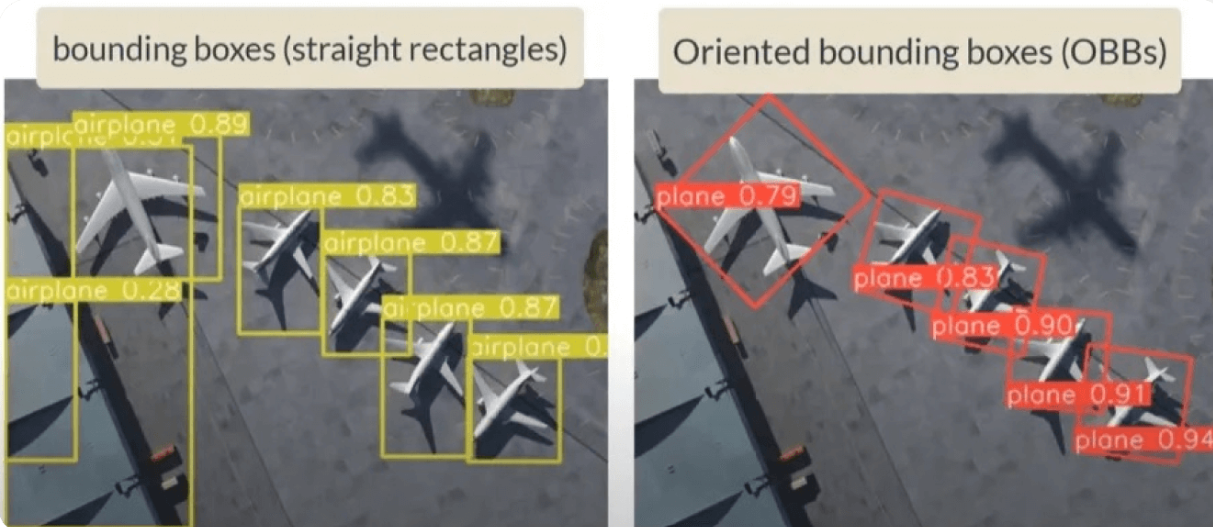
\includegraphics[width=0.7\textwidth]{appendices/images/FigureOBB.png}
    \caption{Comparing normal bounding boxes and oriented bounding boxes. \parencite{ultralytics2024obbblog}.}
    \label{fig:YOLOv8OBBHead}
\end{figure}


